\input{"preamble"}

\usepackage{tabularx}

\hypersetup{
  colorlinks=false,
  linkcolor=black,
  citecolor=black,
  urlcolor=cyan
}

\usepackage[round]{natbib}
\bibliographystyle{plainnat}

\graphicspath{{"./fig/"}}


\def \goml {\href{http://www.ebi.ac.uk/QuickGO/GTerm?id=GO:0051646}{GO:0051646 (mitochondrion localization)}}
\def \gomml {\href{http://www.ebi.ac.uk/QuickGO/GTerm?id=GO:0051659}{GO:0051659} (maintenance of mitochondrion localization)}
\def \gomert {\href{http://www.ebi.ac.uk/QuickGO/GTerm?id=GO:1990456}{GO:1990456} (mitochondrion-ER tethering)}
\def \goeml {\href{http://www.ebi.ac.uk/QuickGO/GTerm?id=GO:0051654}{GO:0051654} (establishment of mitochondrion localization)}
\def \gommaaf {\href{http://www.ebi.ac.uk/QuickGO/GTerm?id=GO:0034642}{GO:0034642} (mitochondrial migration along actin filament)}
\def \goemlmm {\href{http://www.ebi.ac.uk/QuickGO/GTerm?id=GO:0034643}{GO:0034643} (establishment of mitochondrial localization, microtubule mediated)}
\def \goemlma {\href{http://www.ebi.ac.uk/QuickGO/GTerm?id=GO:0034640}{GO:0034640} (establishment of mitochondrion localization by microtubule attachment)}
\def \gomtam {\href{http://www.ebi.ac.uk/QuickGO/GTerm?id=GO:0047497}{GO:0047497} (mitochondrion transport along microtubule) }
\def \goemlimf {\href{http://www.ebi.ac.uk/QuickGO/GTerm?id=GO:0090146}{GO:0090146} (establishment of mitochondrial localization involved in mitochondrial fission)}
\def \goremlimf {\href{http://www.ebi.ac.uk/QuickGO/GTerm?id=GO:0090147}{GO:0090147} (regulation of establishment of mitochondrion localization involved in mitochondrial fission)}
\def \gomd {\href{http://www.ebi.ac.uk/QuickGO/GTerm?id=GO:0048311}{GO:0048311} (mitochondrion distribution)}
\def \goidm {\href{http://www.ebi.ac.uk/QuickGO/GTerm?id=GO:0048312}{GO:0048312} (intracellular distribution of mitochondria)}
\def \gomi {\href{http://www.ebi.ac.uk/QuickGO/GTerm?id=GO:0000001}{GO:0000001} (mitochondrion inheritance)}

\def \SyRO {\href{https://github.com/hyginn/SyRO}{github.com/hyginn/SyRO}}
\def \firstpool {\href{https://github.com/thejmazz/biologicalsystem/blob/master/notebook.md\#user-content-summary-of-first-pool}{notebook}}

\newcommand{\uniprot}[1]{\href{http://www.uniprot.org/uniprot/#1}{#1}}

\begin{document}

\title{
\vspace{-155pt}
\hspace*{-80pt}\includegraphics[width=1.35\linewidth]{"purkinje-neuron-mitochondria"}
Neuronal Mitochondrion Trafficking \\
\small{\textit{BCH441 Project: Defining a System}}
}
\author{Julian Mazzitelli}
\date{Dec. 25, 2015}

\maketitle

\begin{center}
\textit{
The source code, notebook, and data pipeline can be found at
\href{https://github.com/thejmazz/biologicalsystem}{github.com/thejmazz/biologicalsystem}. \\
Cover image (mitochondrion in Purkinje neuron) by Atlas of Ultrastructural Neurocytology\footnote{\href{http://synapses.clm.utexas.edu/atlas/1_1_2_8.stm}{synapses.clm.utexas.edu/atlas/1\_1\_2\_8.stm}}
}
\end{center}

\tableofcontents

\begin{bottompar}
\section{Introduction}

The ``powerhouse of the cell'' as it is so commonly called, the mitochondria is
one of the most vital organelles in eukaryotes. This structure is thought to
have developed through a symbiotic relationship among engulfed prokaryotic cells
and their hosts. As such, it is rooted quite deeply evolutionarily, and one
might expect its proper functioning to be absolutely vital, that is, knock-out
mutants will not survive. This is true - but as we will see, it is not just the
performance of this organelle which is centrally important, but where it is
localized within the cell as well.

\end{bottompar}

Images of isolated mitochondria were first observed in \citeyear{Lincoln1979}
by \citeauthor{Lincoln1979}:

\begin{center}
  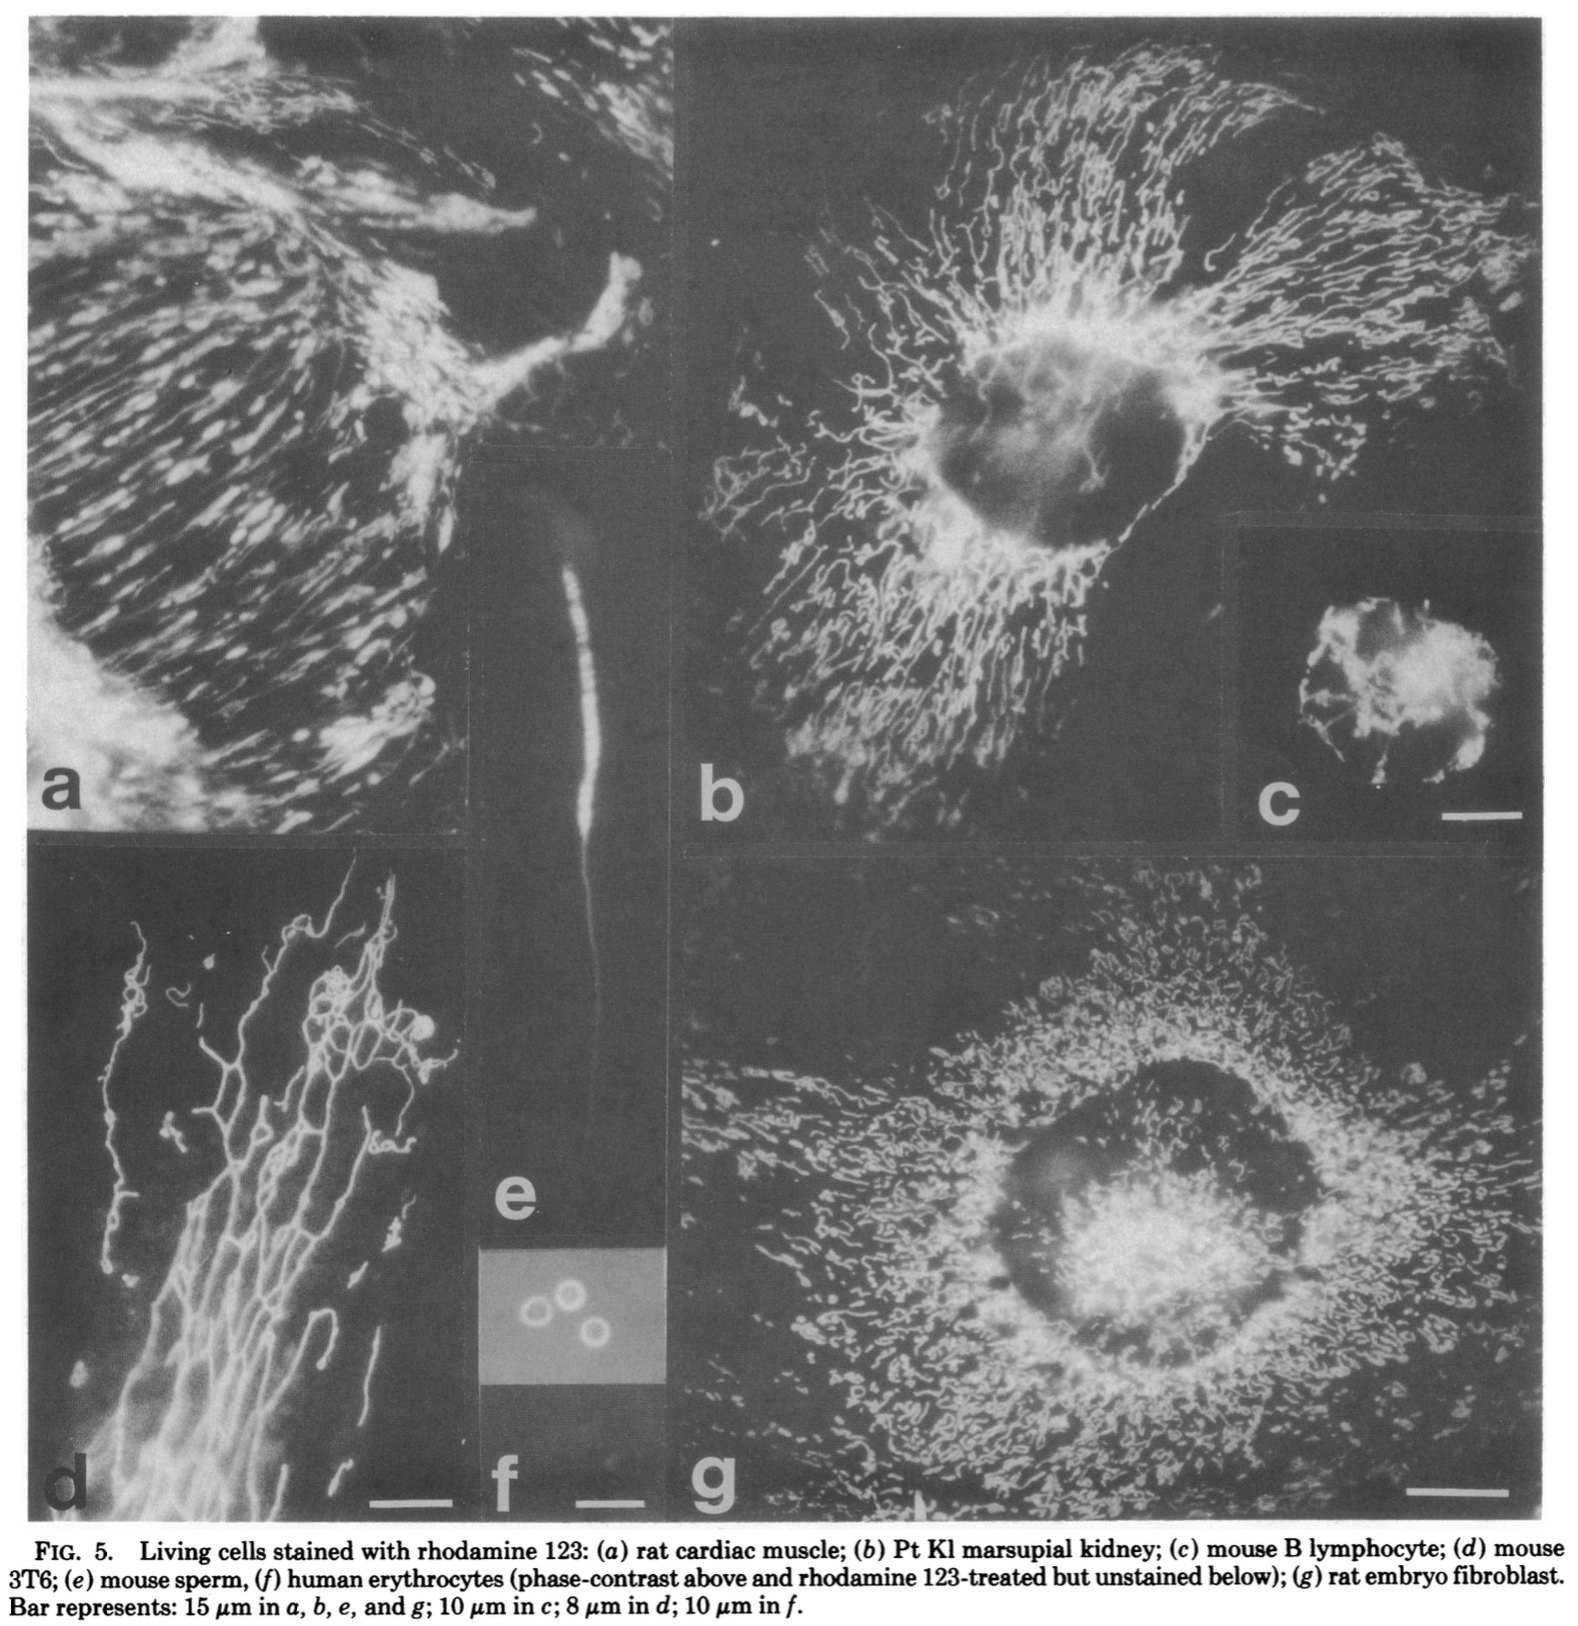
\includegraphics[width=0.6\linewidth]{rhodamine-mitochondria}
\end{center}

\noindent The variety of mitochondrion shape and size is clear, ranging from
globular to filamentous to networked structures. As well, the authors observed
movement during 15-30 sec intervals, between fluorescent and phase-contrast
photographs.

The primary role of a mitochondrion is to supply energy to the cell in the form
of ATP units, through the electron transport chain among the cristae. Where is
that energy needed? Consider highly polar and elongated cells such as neurons.
The cell body of a neuron is distant from its synaptic endings, where as it
happens, large amounts of energy are required for neurotransmitter release and
absorption. Following, we will investigate the \textbf{system} whose
\textbf{functional role} is the \textbf{localization of mitochondrion within
neurons}.

\section{The System}

\begin{tabularx}{\linewidth}{l X}
  \textit{Name} & Localization/Trafficking of mitochondrion within neurons \\
  \textit{Description} & The collective of functional units represented by genes which process signals, transduce these events, initiate, and maintain the actions necessary to transport mitochondrion to distal points along the axon of a neuron. \\
  \textit{Associated GO Terms} & \goml
\end{tabularx}

\begin{itemize}
  \item \gomml
  \begin{itemize}
    \item \gomert
  \end{itemize}
  \item \goemlmm
  \begin{itemize}
    \item \gommaaf
    \item \goemlmm
    \begin{itemize}
      \item \goemlma
      \item \gomtam
    \end{itemize}
    \item \goemlimf
    \begin{itemize}
      \item \goremlimf
    \end{itemize}
  \end{itemize}
  \item \gomd
  \begin{itemize}
    \item \goidm
    \item \gomi
  \end{itemize}
\end{itemize}

Why this system? Originally I was looking into ``mitochondrial localization.''
Amongst the genes returned by the ontology, there appeared those related to
mitochondrial localization during cellular reproduction, transport,
microtubules, tethers, mRNA-binding, and various ``popular'' genes such as
ubiqutins, serum  albumin, leucine-rich repeat serine/threonine-protein kinase,
basic helix-loop-helix protein. There was a fair amount of variety. In order to
gather together a structured list of genes I would need to filter these out, and
to filter these out I would need a functional goal. I decided to choose the
neuronal process because it is one of the most extreme cases of mitochondrial
movement in all cell types, there was a decent amount of related literature
available, some elements of its processes had been recently elecidated, and it
has important neurophysiological consequences. A review by \cite{Reis2009}
explored the atypical Miro GTPases and their role in transporting mitochondria
in neurons. The authors note that abnormal mitochondrial dynamics can contribute
to Amyotropic Lateral Sclerosis (ALS), Huntington's, Parkinson's, and
Alzheimer's diseases. A more recent experiment by \cite{Loss2015} examines the
role of TRAK1 and TRAK2 kinesin adaptor proteins which link mitochondria to
kinesin motor proteins. Furthermore, Miro proeins are expressed in a large
variety of cell types, potentially extending this current analysis to new
domains \citep{Reis2009}.

\subsection{Systems Role Ontology}

To define this system in a structured manner, I considered its functionality
in the context of the Systems Roles Ontology, which can be found at \SyRO:

\begin{center}
  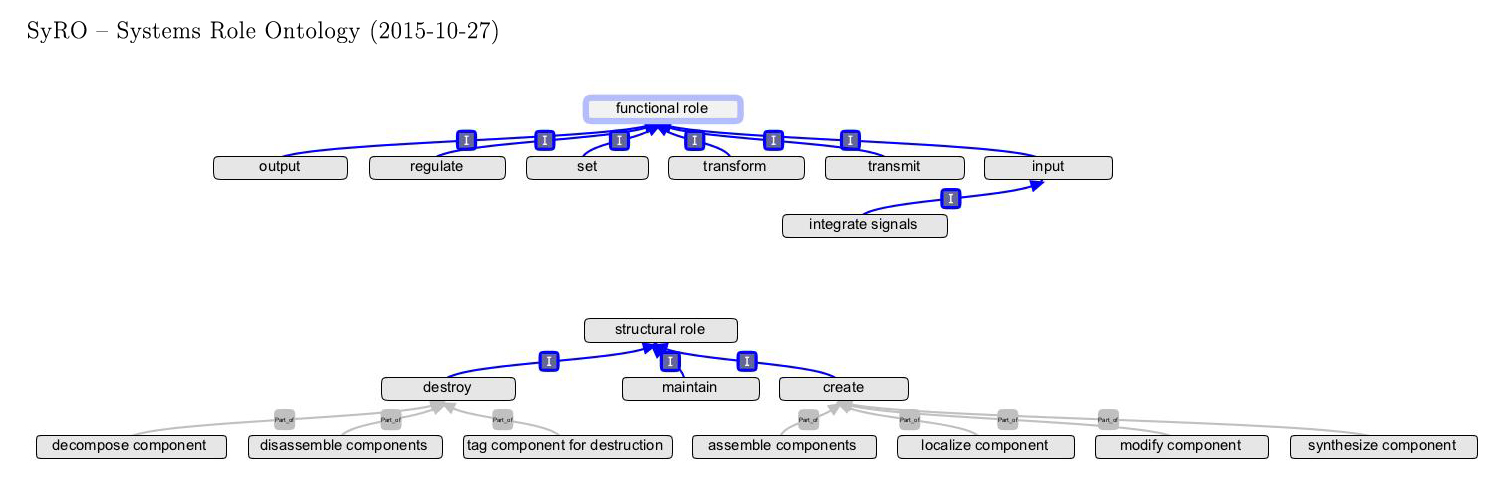
\includegraphics[width=1\linewidth]{SyRO-2015-10-27}
\end{center}

\begin{tabularx}{\linewidth}{l l X}
  \textit{\textcolor{grey}{Name}} & \textit{\textcolor{grey}{ID}} & \textit{\textcolor{grey}{Context Within Neuronal Mitochondrion Localization}} \\
  \textbf{input} & \texttt{16} & compounds or signals prompting the directed movement of mitochondrion \\
  \textbf{integrate signals} & \texttt{22} & machinery which directs input signals/compounds to the system \\
  \textbf{output} & \texttt{21} & mitocondrion transport towards synaptic endings \\
  \textbf{regulate} & \texttt{20} & components which ensure regular mitochondrial motility \\
  \textbf{set} & \texttt{19} & preparing the functional units, ``setting the stage'' as it were  \\
  \textbf{transform} & \texttt{18} & altering the system status so that it may be reversed, stopped, reinstated \\
  \textbf{transmit} & \texttt{17} & the physical machinery to move mitochondria \\
\end{tabularx} \\

These functions collaborate to produce the \textbf{functional role} of
localizing mitochondria \textbf{for the proper functioning of neural
communication}. I will define the bounds of this system as any genes which can
be annotated with the functional role annotations above. Structural role
annotations will be considered second to function, and will be used largely to
describe how that component physically determines its function. With this goal
in mind, I fetched and filtered data from the Gene Ontology Consortium, QuickGO,
UNIPROT, IntAct, and STRING. Those genes which did not make the cut can be seen
through the \textit{Summary of first pool} in my \firstpool.

\section{Gene Collection}

\rowcolors{2}{white}{gray!25}
\begin{tabularx}{\linewidth}{l l X X}
  \textit{Gene} & \textit{Accession} & \textit{Name} & \textit{SyRO} \\
  RHOT2 & \uniprot{Q8IXI1} & Mitochondrial Rho GTPase 2 & integrate, assemble \\
  RHOT1 & \uniprot{Q8IXI2} & Mitochondrial Rho GTPase 1 & integrate, assemble \\
  MGARP & \uniprot{Q8TDB4} & Mitochondria-localized glutamic acid-rich protein & regulate, localize components \\
  TRAK1 & \uniprot{Q9UPV9} & Trafficking kinesin-binding protein 1 & transmit \\
  TRAK2 & \uniprot{Q8IU62} & Trafficking protein, kinesin binding 2 & transmit \\
  MAPT & \uniprot{P10636} & Microtubule-associated protein tau & dissassemble, localize, set \\
  MAP1B & \uniprot{P46821} & Microtubule-associated protein 1B & assemble, integrate signals \\
  TIAM2 & \uniprot{Q8IVF5} & T-lymphoma invasion and metastasis-inducing protein 2 & localize, modify, integrate signals \\
  TTL & \uniprot{Q8NG68} & Tubulin--tyrosine ligase & modify, assemble \\
  GAN & \uniprot{Q9H2C0} & Gigaxonin & decompose, tag, regulate \\
  KIF1B & \uniprot{O60333} & Kinesin-like protein KIF1B & transmit, transform, maintain \\
  AIM21 & \uniprot{P40563} (yeast) & Altered inheritance of mitochondria protein 21 & assemble, localize, integrate, transmit \\
  MYO19 & \uniprot{Q5SV80} (mouse) & Unconventional myosin-XIX & maintain, transform \\
  MDM10 & \uniprot{P18409} (yeast) & Mitochondrial distribution and morphology protein 10 & regulate, integrate, assemble, localize \\
  PFDNS & \uniprot{Q99471} & Prefoldin subunit 5 & regulate, integrate, assemble, localize \\
  MDM12 & \uniprot{Q92328} (yeast) & Mitochondrial distribution and morphology protein 12 & regulate, integrate, assemble, localize \\
  MILT & \uniprot{Q960V3} (fly) & Trafficking kinesin-binding protein milt & assemble, localize, output, set \\
  CLUH & \uniprot{I3L2B0} & Clustered mitochondria protein homolog & localize, set \\
  BHLHA15 & \uniprot{Q7RTS1} & Class A basic helix-loop-helix protein 15 & synthesize, assemble, set \\
  MTM1 & \uniprot{Q13496} & Myotubularin & set, localize, modify \\
  MSTO1 & \uniprot{Q9BUK6} & Protein misato homolog 1 & set, maintain, transform \\
  ATCAY & \uniprot{Q86WG3} & Caytaxin & regulate, assemble, transmit \\
  KLCA1 & \uniprot{Q07866} & Kinesin light chain 1 & integrate, assemble \\
\end{tabularx}

\bibliography{biblio}


\end{document}
